% !TeX root = ../../latex-talk.tex

\part{像模像样 \LaTeX{}}

\section{\TikZ{}}

\begin{frame}
  \frametitle{绘何物为\footnote{中文译者 Hansimov \link{https://github.com/Hansimov/pgfmanual-zh},中文拼音 Hu\`i \textbf{h}\'e w\textbf{\`u} w\'e\textbf{i}。}}

  \note[item]{中文译名来自 Hansimov 看起来已经弃坑的《\TikZ{} \& \textsc{pgf} 中文手册》,可以催催他继续翻译这一千多页的大部头!}

  \begin{description}
    \item[\TikZ{}] (\alert{T}i\textit{k}Z \alert{i}st \textit{\alert{k}ein} \alert{Z}eichenprogramm\footnote{中文含义是“\TikZ{} 不是一个绘图程序”,德文跟随 \textbf{G}NU's \textbf{N}ot \textbf{U}nix! 传统。}) 定义了一些 \TeX{} 中的绘图命令,基础语法神似矢量字体设计语言 \hologo{METAFONT} 指令。
    \item[\pgf{}] (\alert{p}ortable \alert{g}raphics \alert{f}ormat\note[item]{pgf 很像 PDF 的全称:\textbf{p}ortable \textbf{d}ocument \textbf{f}ormat。}) 组成了 \TikZ{} 的基本层。\cls{beamer} 的一些机制也是基于此底层实现的。
  \end{description}

  \begin{figure}
    
\includegraphics[width=0.75\textwidth]{support/figures/tikzlings.pdf}
    \caption{\TikZ{}lings 绘制的小动物 \link{https://github.com/samcarter/tikzlings}}
  \end{figure}

  \note[item]{\LaTeX3 中的 \texttt{l3draw} \link{https://github.com/latex3/latex3/tree/main/l3experimental/l3draw} 妄图统一这种绘图宏包,目前仍处于实验阶段。}
\end{frame}

\begin{frame}[fragile,label=tikz]
  \frametitle{引入 \TikZ{}}
  \begin{columns}
    \begin{column}{0.4\textwidth}
      
      \only<1>{
        可以直接在文档导言区使用 \TikZ{} 包 \link{https://mirrors.sjtug.sjtu.edu.cn/CTAN/graphics/pgf/base/doc/pgfmanual.pdf},或者采用 \cls{standalone} 文档类。 

        \note[item]{如果需要使用中文,还需要添加 \pkg{ctex} 宏包。}
      }

      \only<2>{
        引入 \TikZ{} 后,使用 \env{tikzpicture} 环境开始绘制。
      }

      \only<3>{
        \TikZ{} 命令需要以分号结尾。\cmd{node} 命令用于创建节点,还可以为该节点标记标签以便后续引用。
      }

      \only<4>{
        \cmd{draw} 用来描边,\opt{edge} 用来指示这是一条线段,参数 \opt{->} 用来说明这是一个箭头。紧随其后可以添加线段上的节点,\opt{above}, \opt{below}, \opt{left}, \opt{right} 可以用来指示相对位置。
      }

      \only<5>{
        \opt{draw} 参数用于对节点描边。
      }

      \begin{center}
        \begin{tikzpicture}
          \only<1-4>{
            \node (v1) at (0,0) {\only<3>{\color{red}}$x$};
            \node (v2) at (1,0) {\only<3>{\color{red}}$a$};
          }
          \only<5>{
            \node[draw] (v1) at (0,0) {\only<3>{\color{red}}$x$};
            \node[draw] (v2) at (1,0) {\only<3>{\color{red}}$a$};
          }
          \only<1-3,5>{\draw[->]  (v1) edge node [above] {$z$} (v2);}
          \only<4>{\draw[->,red]  (v1) edge node [above,red] {$z$} (v2);}
        \end{tikzpicture}
      \end{center}
    \end{column}
    \begin{column}{0.6\textwidth}
      \begin{codeblock}[]{使用 \TikZ{}}
|\highlightline<1>|\documentclass[tikz]{standalone}
\begin{document}
|\highlightline<2>|\begin{tikzpicture}
|\highlightline<3,5>|  \node|\only<5>{[draw]}| (v1) at (0,0) {$x$};
|\highlightline<3,5>|  \node|\only<5>{[draw]}| (v2) at (1,0) {$a$};
|\highlightline<4>|  \draw  (v1) edge[->] 
|\highlightline<4>|    node [above] {$z$} (v2);
|\highlightline<2>|\end{tikzpicture}
||\end{document}
      \end{codeblock}
    \end{column}
  \end{columns}
\end{frame}

\begin{frame}[fragile]
  \frametitle{\only<1-3>{循环}\only<4>{样式}}
  \begin{columns}
    \begin{column}{0.4\textwidth}

      \only<1>{
        \begin{figure}
          \centering
          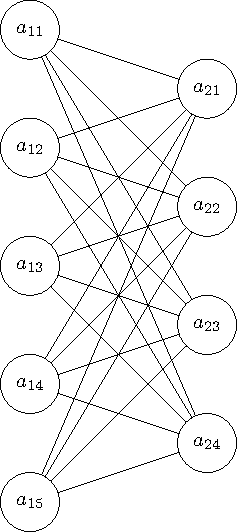
\includegraphics[height=0.6\textheight]{support/figures/neural.pdf}
        \end{figure}

        \note{绘制神经网络图像可能是非常适合 \TikZ{} 干的事情了,你说用 PowerPoint 繁琐的线段连接估计需要借助插件才能比较方便地实现。使用其他非编程性绘图工具都是比较头疼的事情。}
      }

      \only<2-3>{

        \pgf{} 提供 \cmd{foreach} 用来创建循环体,以绘制繁琐且结构类似的图。

        \vspace{4ex}

        \onslide<3>{
          \cmd{foreach} 可以嵌套使用。
        }
      }

      \only<4>{
        \TikZ{} 提供 \cmd{tikzstyle} 命令用于设定一个样式别称。\note{类似于 HTML 中的 class 然后通过 CSS 设定样式。}之后的节点或者边就可以直接套用该样式。

        \note{更多方法参见手册,内容非常多。}
      }

    \end{column}
    \begin{column}{0.6\textwidth}
      \begin{codeblock}[basicstyle=\ttfamily\scriptsize]{神经网络}
\documentclass[tikz]{standalone}
\begin{document}
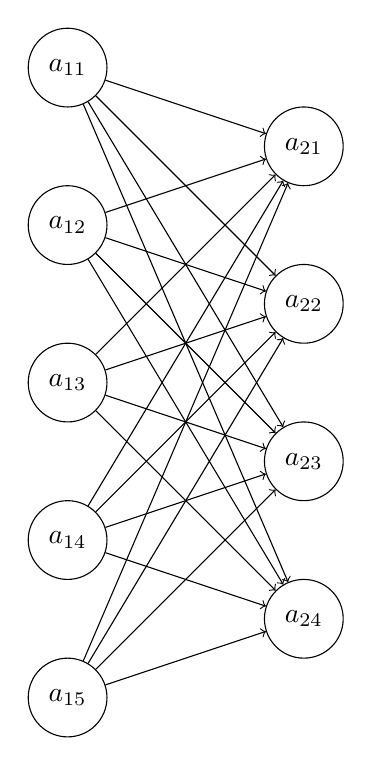
\begin{tikzpicture}
|\highlightline<4>|\tikzstyle{neuron}=[circle,draw,minimum width=1cm];
|\highlightline<2>|\foreach \x in {1,...,5} {
|\highlightline<4>|  \node[neuron] (a\x) at (0,-2*\x) {$a_{1\x}$};
}
\foreach \y in {1,...,4} {
|\highlightline<4>|  \node[neuron] (b\y) at (3,-1-2*\y) {$a_{2\y}$};
}
|\highlightline<3>|\foreach \x in {1,...,5} {
|\highlightline<3>|  \foreach \y in {1,...,4} {
    \draw (a\x) edge[->] (b\y);
  }
}
\end{tikzpicture}
\end{document}
      \end{codeblock}
    \end{column}
  \end{columns}
\end{frame}

\begin{frame}[fragile]
  \frametitle{思维导图}
  \begin{columns}
    \begin{column}{0.4\textwidth}
      还可以通过 \cmd{usetikzlibrary} 调用内置库来绘制更多类型的图像。
      
      \note{比如 \pkg{mindmap} 可以用来绘制思维导图。}

      \note{声明该 \env{tikzpicture} 为 \opt{mindmap} 类型,并使用 \opt{child} 指示子级,一个父级可以跟多个子级,子级可以嵌套子级。\opt{grow} 参数用来指示旋转角度,最后需要用分号结束。}

      \begin{figure}
        \centering
        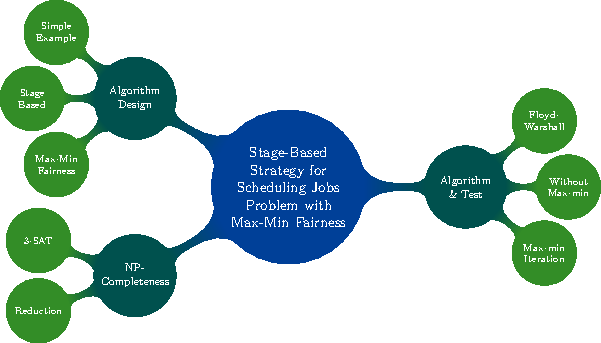
\includegraphics[height=0.35\textheight]{support/figures/mindmap.pdf}
        \caption{\ttfamily \pkg{mindmap} (tikzlibrary)}
      \end{figure}
    \end{column}
    \begin{column}{0.6\textwidth}
      \begin{codeblock}[]{\pkg{mindmap} 框架}
\documentclass[tikz]{standalone}
|\highlightline|\usetikzlibrary{mindmap}
\begin{document}
\begin{tikzpicture}[mindmap, concept color=blue]
\node [concept] {Parent} 
child [concept color=gray, grow=150] {
  node [concept] {Child1}}
child [concept color=gray, grow=0] {
  node [concept] {Child2}};
\end{tikzpicture}
\end{document}
      \end{codeblock}
    \end{column}
  \end{columns}

  \note{\pkg{mindmap} 库是 \TikZ{} 中非常 iconic 的一个库。}
\end{frame}

\begin{frame}
  \frametitle{\TikZ{}Edt}
  \includeinlinelogo{support/images/tikzedt.png} \TikZ{}Edt \link{http://www.tikzedt.org/} 是一款半图形化的即时绘图编辑器,在 \faWindows{} 上工作较好。

  \begin{columns}
    \begin{column}{0.4\textwidth}
      \begin{itemize}
        \item 善用工具栏功能 \link{http://www.tikzedt.org/doc.html}
        
        
\includegraphics[width=\linewidth]{support/images/tooltip.png}
        \item 开始时会提示生成缩略图
        
        {\tiny Compilation $\blacktriangleright$ Compile snippet thumbnails}
        \item 如果有时编译不成功了,尝试重新预编译头
        
        {\tiny Compilation $\blacktriangleright$ (Re-)Generate precompiled headers}
        \item 可以更改头文件
        
        {\tiny Settings $\blacktriangleright$ Compiler}
      \end{itemize}
    \end{column}
    \begin{column}{0.6\textwidth}
      \begin{figure}
        \centering
        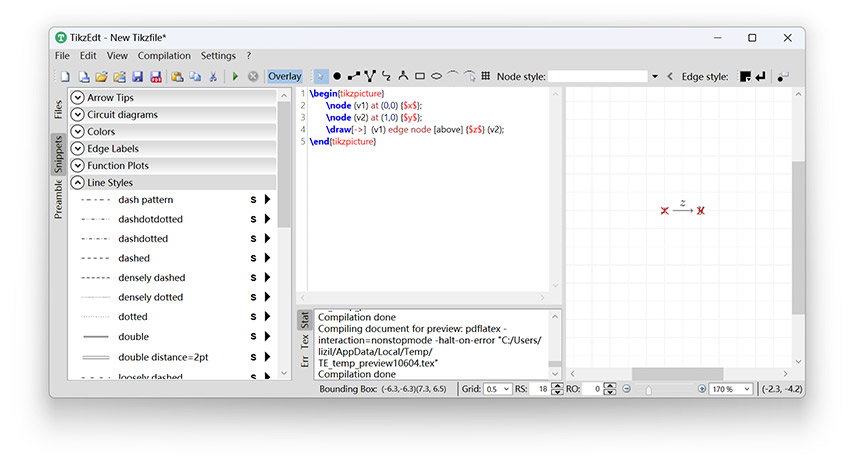
\includegraphics[height=0.5\textheight]{support/images/tikzedtui.jpg}
        \caption{\TikZ{}Edt 界面}
      \end{figure}
    \end{column}
  \end{columns}

  \note[item]{框架基于 Windows Presentation Foundation (WPF),代码开源于 Google Code。2014 年,该项目伴随着这个开源代码平台的终结也开发停止,作者跑路。其适配的 \faApple{} 版本由于跟不上 Mac OS 的更新似乎不再可用,在 \faLinux{} 上更趋向于一种模拟。本人希望在未来有空的时候将其从 .NET Framework 迁移到 .NET Core 上,修改一些脚本文件,以原生跨平台,主要看微软在迁移层面的表现(一般挺好)(本人也对 WPF 较为熟悉,但是这个框架也已慢慢地 deprecated,很多年前是比较流行的,主要这个是 \faWindows{} 专有框架)。}

  \note[item]{\faLinux{}\faApple{} 用户可能本身就更熟悉代码编写的方式,或者转向 Inkscape,以及希望 \TeX{}\textsc{macs} 越来越好(其自带的绘图编辑器看起来也很优秀),这样就可以直接所见即所得了。}
\end{frame}

\section{PGFPlots}

\begin{frame}[fragile]
  \frametitle{PGFPlots}
  \begin{columns}
    \begin{column}{0.4\textwidth}

      \only<1>{
        \pgfplots{} \link{https://mirrors.sjtug.sjtu.edu.cn/CTAN/graphics/pgf/contrib/pgfplots/doc/pgfplots.pdf} 是 \pgf{}/\TikZ{} 的衍生宏包,用于生成高质量中等数据规模的统计图。

        \begin{center}
          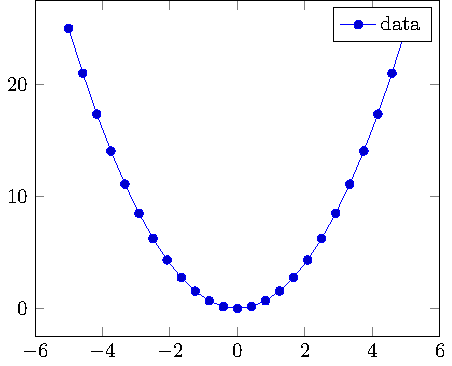
\includegraphics[width=0.75\textwidth]{support/figures/pgfplots.pdf}
        \end{center}
      }

      \only<2>{
        引入 \pgfplots{} 包,然后通过 \cmd{pgfplotsset} 设定版本和其他全局设定。
      }

      \only<3>{
        \env{axis} 环境用于插入 \pgfplots{} 统计图。
      }

      \only<4>{
        \cmd{addplot} 命令用于新建一个数据序列,其后不跟类型的情况下为关于 $x$ 的函数图像。

        \begin{table}
          \centering
          \footnotesize
          \begin{tabular}{>{\ttfamily}ll}
            \cmd{addplot} & 函数 \\
            \cmd{addplot} coordinates & 坐标点 \\
            \cmd{addplot} table & 文件表格 \\
          \end{tabular}
        \end{table}
      }

      \only<5>{
        \cmd{legend} 用于创建图例,使用逗号分隔每个序列的名称。
      }

    \end{column}
    \begin{column}{0.6\textwidth}
      
      \begin{codeblock}[]{使用 \pgfplots{}}
\documentclass[tikz]{standalone}
|\highlightline<2>|\usepackage{pgfplots}
|\highlightline<2>|\pgfplotsset{compat=newest}
\begin{document}
|\highlightline<3>|\begin{axis}
|\highlightline<4>|  \addplot {x^2};
|\highlightline<5>|  \legend{data,};
|\highlightline<3>|\end{axis}
||\end{document}
      \end{codeblock}
      
    \end{column}
  \end{columns}
\end{frame}

\begin{frame}[fragile]
  \frametitle{PGFPlotsTable}

  \begin{columns}
    \begin{column}{0.4\textwidth}
      
      \only<1>{
        \pgfplotstable{} \link{https://mirrors.sjtug.sjtu.edu.cn/CTAN/graphics/pgf/contrib/pgfplots/doc/pgfplotstable.pdf} 是用于数据处理的子包,可以用来从文件排印表格。

        \begin{center}
          \includepdflarge{support/examples/pgfplotstable.pdf}
        \end{center}
      }

      \only<2>{
        \cmd{pgfplotstableset} 用于设定全局设置。这里设定了默认使用 CSV 文件,表格采用标准三线表格式。

        \begin{block}{\faInfo{}}
          SJTUBeamer 已经预先设置了这些格式。
        \end{block}
      }

      \only<3>{
        \cmd{pgfplotstabletypeset} 用于从文件排印表格。这样你的 CSV 文件就可以通过 Excel 软件编辑与处理。
        \note{又一层内容与格式分离!}

        \begin{block}{\faExclamationTriangle}
          含有中文内容的表格需要使用 \hologo{XeLaTeX} 编译!
        \end{block}
      }

    \end{column}
    \begin{column}{0.6\textwidth}
      
      \begin{codeblock}[]{使用 \pgfplotstable{}}
\documentclass{ctexart}
\usepackage{booktabs}
|\highlightline<1>|\usepackage{pgfplotstable}
\pgfplotsset{compat=newest}
|\highlightline<2>|\pgfplotstableset{
  col sep=comma,
  every head row/.style={before row=\toprule,after row=\midrule},
  every last row/.style={
    after row=\bottomrule},
}
\begin{document}
|\highlightline<3>|  \pgfplotstabletypeset[]{data.csv}
||\end{document}
      \end{codeblock}
      
    \end{column}
  \end{columns}

\end{frame}

\begin{frame}
  \frametitle{PGFPlotsEdt}
  \includeinlinelogo{support/images/pgfplotsedt.pdf} PGFPlotsEdt \link{https://logcreative.github.io/PGFPlotsEdt/?lang=cn} 是一款基于 \pgfplots{} 的统计绘图编辑器,基于 \faVuejs{} 开发。

  \begin{columns}
    \begin{column}{0.4\textwidth}
      \begin{itemize}
        \item 顶部按钮提供了一些示例。
        \item 推荐首先在设定中设置好参数(比如三维)。
        \item 可以设置坐标系相关样式。
        \item 直接按下 \faExclamationTriangle{} 手动编辑代码。
        \note{按下没有回头路。因为回头路我没做好。}
      \end{itemize}
    \end{column}
    \begin{column}{0.6\textwidth}
      \begin{figure}
        \centering
        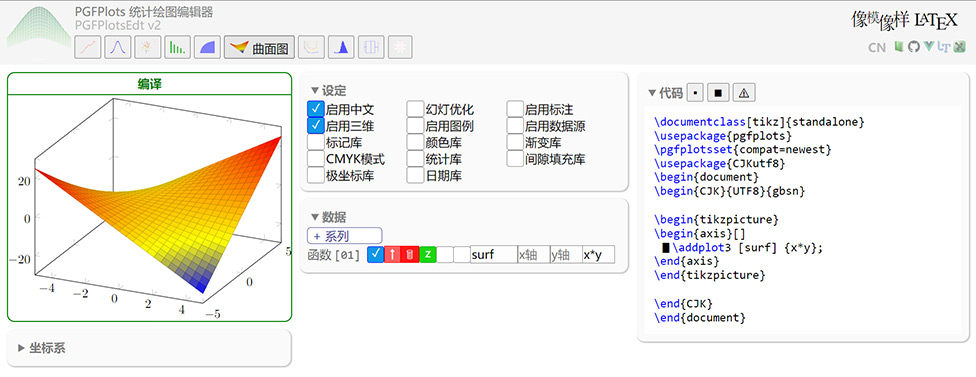
\includegraphics[height=0.4\textheight]{support/images/pgfplotsedtui.jpg}
        \caption{PGFPlotsEdt 界面}
      \end{figure}
    \end{column}
  \end{columns}

  \note{当年是想做个跟 \TikZ{}Edt 类似的软件,用于快速生成统计图代码。也想过使用 Qt 写,当然后面放弃了,转向编写网页应用。当时本人还没有什么服务器,就写了个纯前端。}

  \note{我为什么后来想翻译 Learn\LaTeX{}.org,也是因为我看到了它使用的编辑器框架与轻量级编译服务,非常适合用来开发小型软件,PGFPlotsEdt 也就是这个思想的实践。}
\end{frame}

\begin{frame}
  \frametitle{PGFPlotsEdt 帮助我完成物理实验报告图...}
  \begin{columns}
    \begin{column}{0.25\textwidth}
      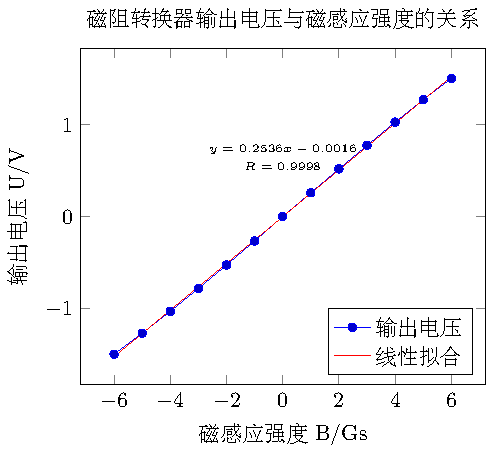
\includegraphics[width=\linewidth]{support/pgfplots/a.pdf}
      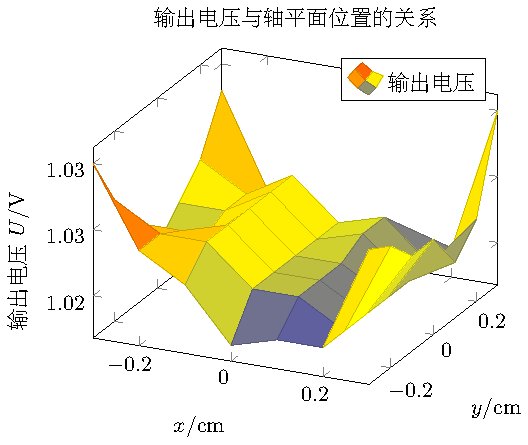
\includegraphics[width=\linewidth]{support/pgfplots/b.pdf}
    \end{column}
    \begin{column}{0.50\textwidth}
      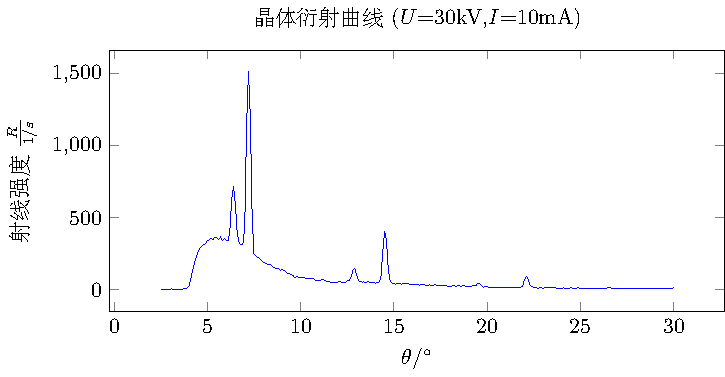
\includegraphics[width=\linewidth]{support/pgfplots/c.pdf}
      \begin{columns}
        \begin{column}{0.5\linewidth}
          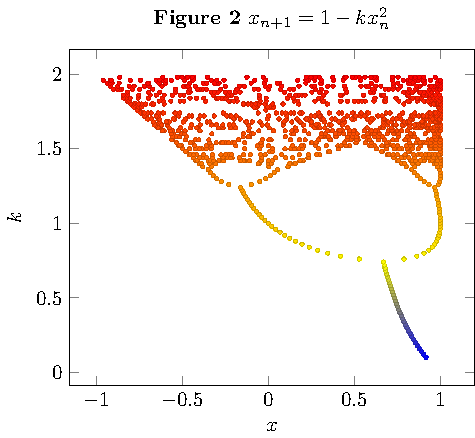
\includegraphics[width=\linewidth]{support/pgfplots/d.pdf}
        \end{column}
        \begin{column}{0.5\linewidth}
          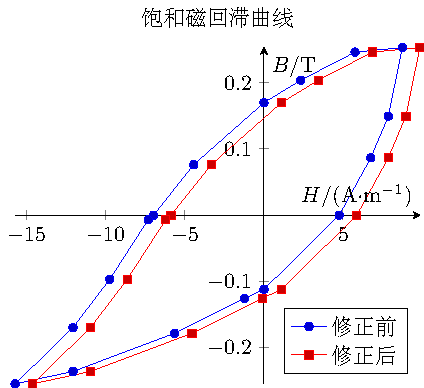
\includegraphics[width=\linewidth]{support/pgfplots/e.pdf}
        \end{column}
      \end{columns}
    \end{column}
    \begin{column}{0.25\textwidth}
      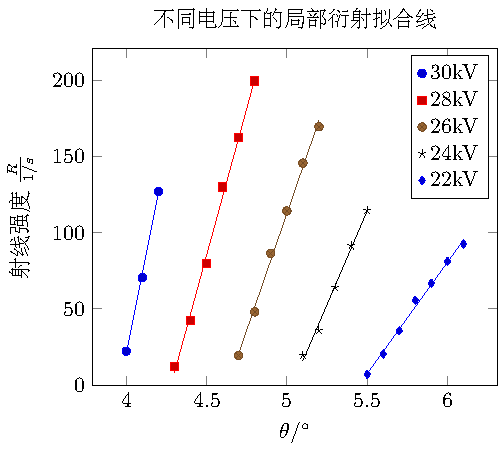
\includegraphics[width=\linewidth]{support/pgfplots/f.pdf}
      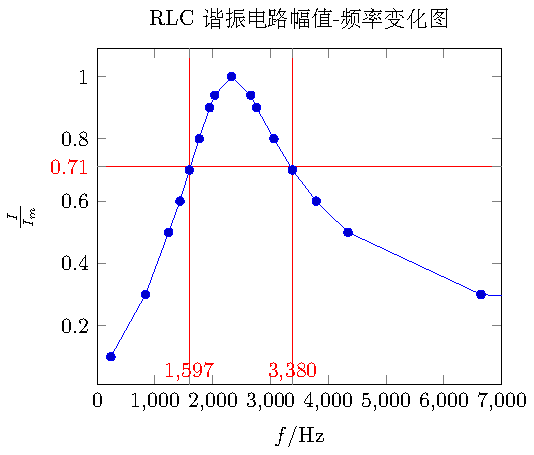
\includegraphics[width=\linewidth]{support/pgfplots/g.pdf}
    \end{column}
  \end{columns}
\end{frame}

\begin{frame}
  \frametitle{更多可能}

  \begin{columns}
    \begin{column}{0.58\textwidth}
      \begin{itemize}
        \item \TikZ{} 还内置很多的库可供使用!
        \item \TikZ{} 还有很多的衍生库可供使用!
        \note[item]{不只是 \pgfplots{}。}
        \item 推荐使用 \cls{standalone} 文档类编译再插入。
        \item 内存不足时需要使用 \hologo{LuaLaTeX} 编译。
        \note[item]{\hologo{LuaLaTeX} 使用了动态内存。之前的一个分形图就是因为需要大量的内存需要 \hologo{LuaLaTeX} 编译。}
        \item 使用 \pkg{external} 库缓存也是可行的。
        \item 更多内容请见手册\footnotemark。
      \end{itemize}
    \end{column}
    \begin{column}{0.42\textwidth}
      \begin{figure}
        \begin{tikzpicture}[scale=0.7,every node/.style={scale=0.7}]
          \node[draw,fill=white] (v1) at (-1.5,0) {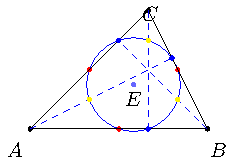
\includegraphics[scale=0.7]{support/figures/tkzeuclide.pdf}};
          \node[draw,fill=white] at (1.5,-2) {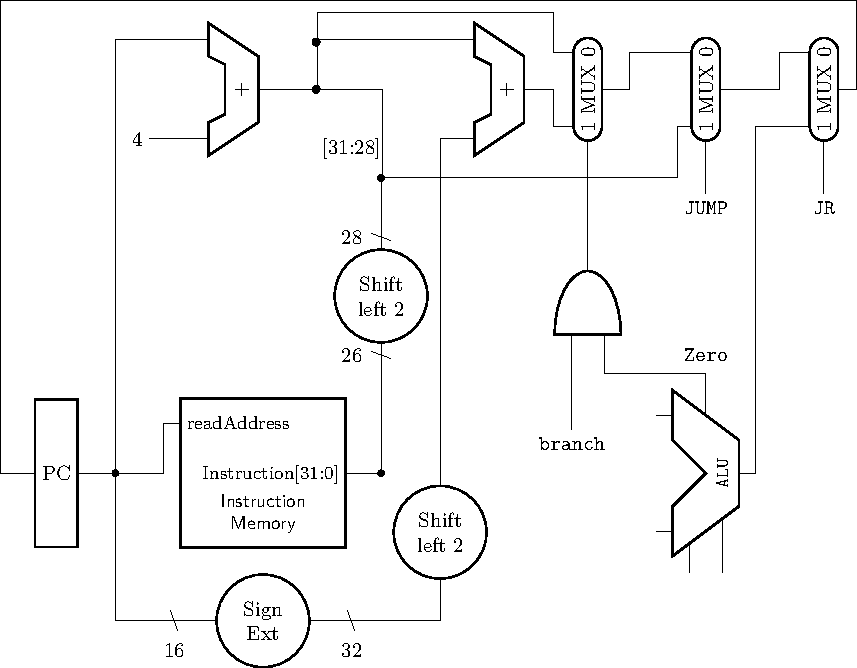
\includegraphics[scale=0.3]{support/figures/circuitikz.pdf}};
          \node[draw,fill=white] at (-1.5,-3) {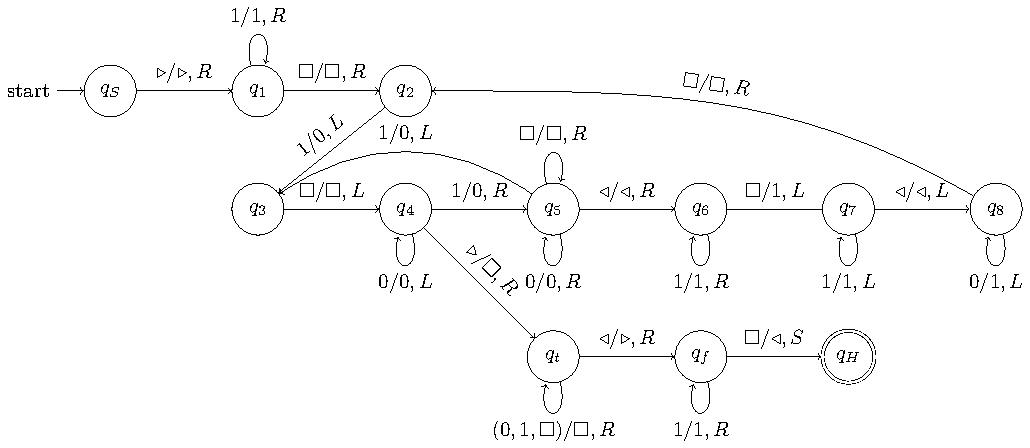
\includegraphics[scale=0.3]{support/figures/automata.pdf}};
        \end{tikzpicture}
        \caption{\ttfamily tkz-euclide \link{http://mirrors.sjtug.sjtu.edu.cn/CTAN/macros/latex/contrib/tkz/tkz-euclide/doc/tkz-euclide.pdf}, circuitikz \link{https://mirrors.sjtug.sjtu.edu.cn/CTAN/graphics/pgf/contrib/circuitikz/doc/circuitikzmanual.pdf}, automata (tikzlibrary)}
      \end{figure}
    \end{column}
  \end{columns}

  \footnotetext{(中文版)\LaTeX{} 工作室.
  \TikZ{} \& \pgf{} 手册 (3.1.5b) 笔记[EB/OL].
  2020. \link{https://www.latexstudio.net/archives/51804.html}}
  
  \note[item]{看文档需要使用 texdoc pgf,这个笔记大略翻译了很多内容。\LaTeX{} 工作室的网站上也有很多 \TikZ{} 的 fancy 内容,感兴趣的可以参考。}

  \note[item]{可以做的很 fancy,也可以用它很基本的功能。因为有一种职业叫科技绘图,这种图形约是符合要求的矢量图。\TikZ{} 的意义在于提供了一种 inline 绘图的方式,有助于管理工程,过早优化万恶之源,这样的方式有助于减少重新绘制的可能。}
  
\end{frame}